%%%%%%%%%%%%%%%%%%%%%%%%%%%%%%%%%%%%%%%%%
% Short Sectioned Assignment
% LaTeX Template
% Version 1.0 (5/5/12)
%
% This template has been downloaded from:
% http://www.LaTeXTemplates.com
%
% Original author:
% Frits Wenneker (http://www.howtotex.com)
%
% License:
% CC BY-NC-SA 3.0 (http://creativecommons.org/licenses/by-nc-sa/3.0/)
%
%%%%%%%%%%%%%%%%%%%%%%%%%%%%%%%%%%%%%%%%%

%----------------------------------------------------------------------------------------
%	PACKAGES AND OTHER DOCUMENT CONFIGURATIONS
%----------------------------------------------------------------------------------------

\documentclass[paper=a4, fontsize=11pt]{scrartcl} % A4 paper and 11pt font size

\usepackage[T1]{fontenc} % Use 8-bit encoding that has 256 glyphs
\usepackage{fourier} % Use the Adobe Utopia font for the document - comment this line to return to the LaTeX default
\usepackage[english]{babel} % English language/hyphenation
\usepackage{amsmath,amsfonts,amsthm} % Math packages

\usepackage{lipsum} % Used for inserting dummy 'Lorem ipsum' text into the template

\usepackage{sectsty} % Allows customizing section commands
\allsectionsfont{\centering \normalfont\scshape} % Make all sections centered, the default font and small caps

\usepackage{fancyhdr} % Custom headers and footers

% use for graph
\usepackage{graphicx} 
\usepackage{subfigure}
\usepackage{caption}
\usepackage{float} 

\pagestyle{fancyplain} % Makes all pages in the document conform to the custom headers and footers
\fancyhead{} % No page header - if you want one, create it in the same way as the footers below
\fancyfoot[L]{} % Empty left footer
\fancyfoot[C]{} % Empty center footer
\fancyfoot[R]{\thepage} % Page numbering for right footer
\renewcommand{\headrulewidth}{0pt} % Remove header underlines
\renewcommand{\footrulewidth}{0pt} % Remove footer underlines
\setlength{\headheight}{13.6pt} % Customize the height of the header

\numberwithin{equation}{section} % Number equations within sections (i.e. 1.1, 1.2, 2.1, 2.2 instead of 1, 2, 3, 4)
\numberwithin{figure}{section} % Number figures within sections (i.e. 1.1, 1.2, 2.1, 2.2 instead of 1, 2, 3, 4)
\numberwithin{table}{section} % Number tables within sections (i.e. 1.1, 1.2, 2.1, 2.2 instead of 1, 2, 3, 4)

\setlength\parindent{0pt} % Removes all indentation from paragraphs - comment this line for an assignment with lots of text

%----------------------------------------------------------------------------------------
%	TITLE SECTION
%----------------------------------------------------------------------------------------

\newcommand{\horrule}[1]{\rule{\linewidth}{#1}} % Create horizontal rule command with 1 argument of height

\title{	
\normalfont \normalsize 
\textsc{University College cork} \\ [25pt] % Your university, school and/or department name(s)
\horrule{0.5pt} \\[0.4cm] % Thin top horizontal rule
\huge The ethical issues in the use of AI in healthcare \\ % The assignment title
\horrule{2pt} \\[0.5cm] % Thick bottom horizontal rule
}

\author{Kai Deng} % Your name

\date{\normalsize\today} % Today's date or a custom date


\begin{document}
\maketitle % Print the title

%----------------------------------------------------------------------------------------
%	PROBLEM 1
%----------------------------------------------------------------------------------------

\section{Introduction}

In the 21st century, advancements in theory and computational power have rapidly propelled 
artificial intelligence (AI), especially in healthcare, drawing significant investments (see Figures 1.1 and 1.2). 
Proponents believe AI can enhance diagnostic accuracy, extend care to remote areas, and save doctors' 
time for more patient interaction \cite{frostPublicViewsEthical2022}. However, AI also brings with a 
colossally abundant number of ethical problem in healthcare area. This text will explore these issues' 
in Privacy and data protection, Transparency and Trust, MResponsibility and Accountability angle and give some suggestings.

\begin{figure}[H]
    \centering
    \begin{minipage}[t]{0.48\linewidth}
        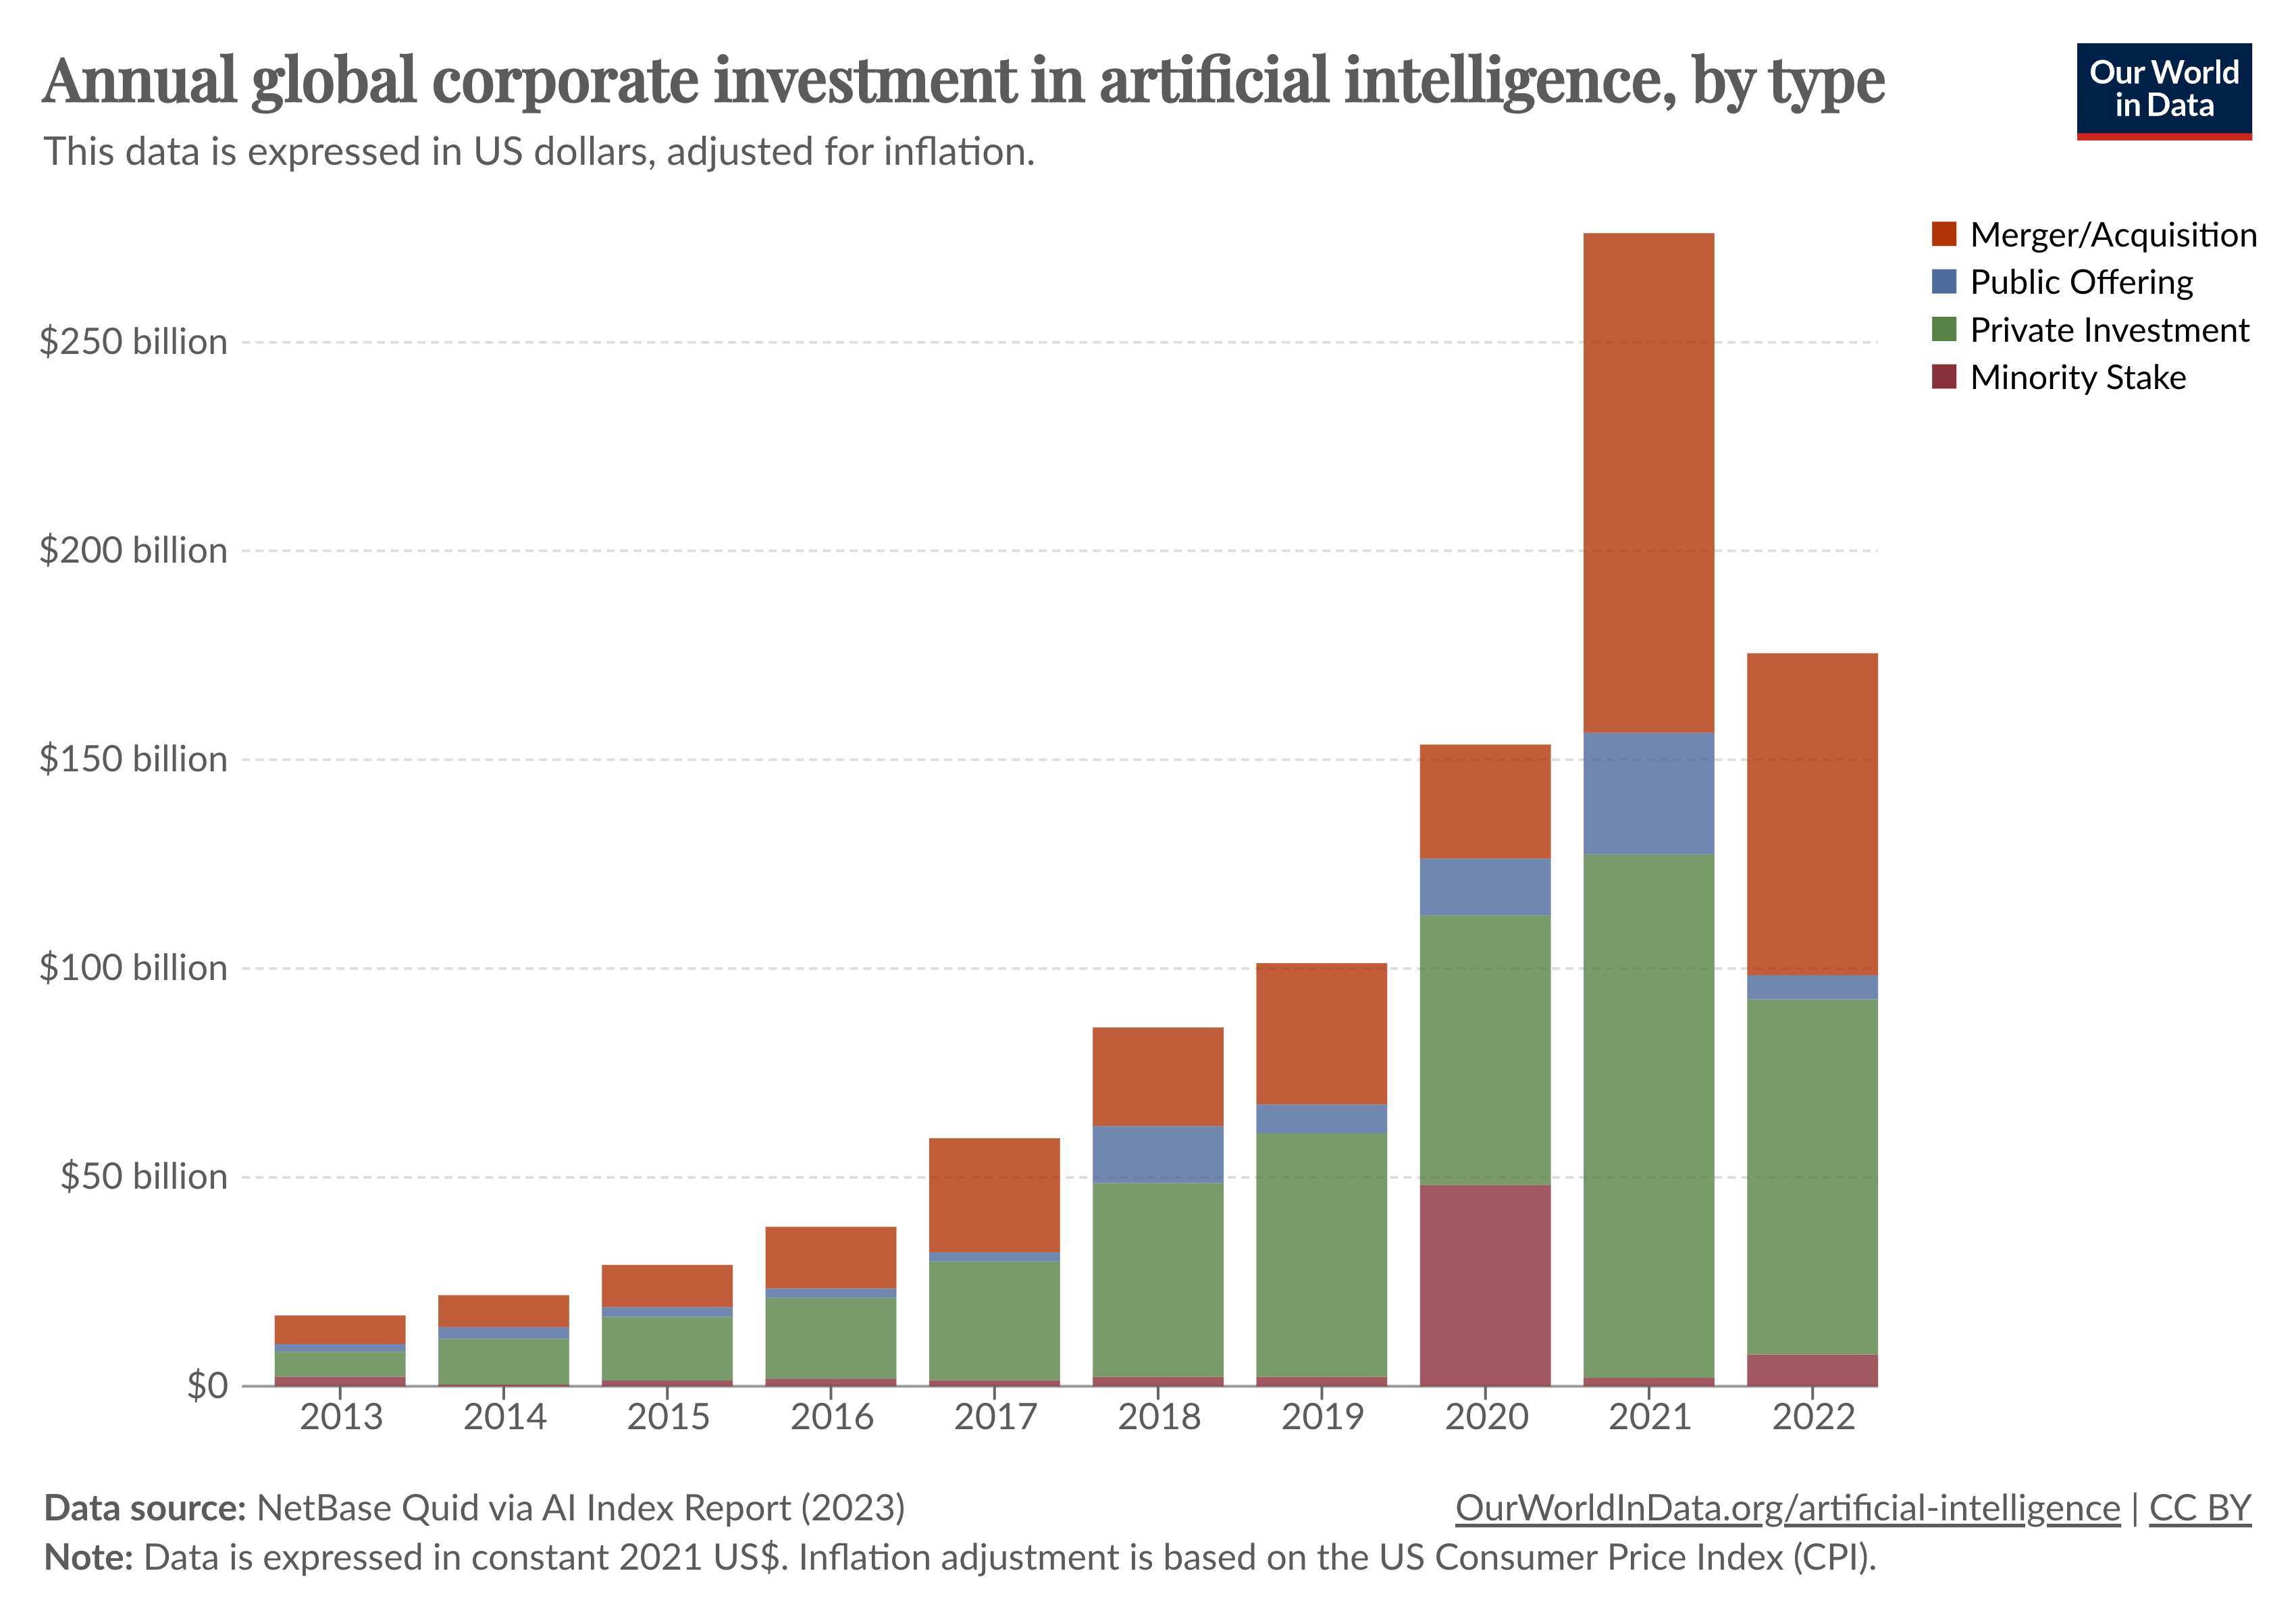
\includegraphics[width=\linewidth]{./data/investment_by_type.png}
        \caption{Annual investment in AI by type}
        \label{fig:investment}
    \end{minipage}\hfill
    \begin{minipage}[t]{0.48\linewidth}
        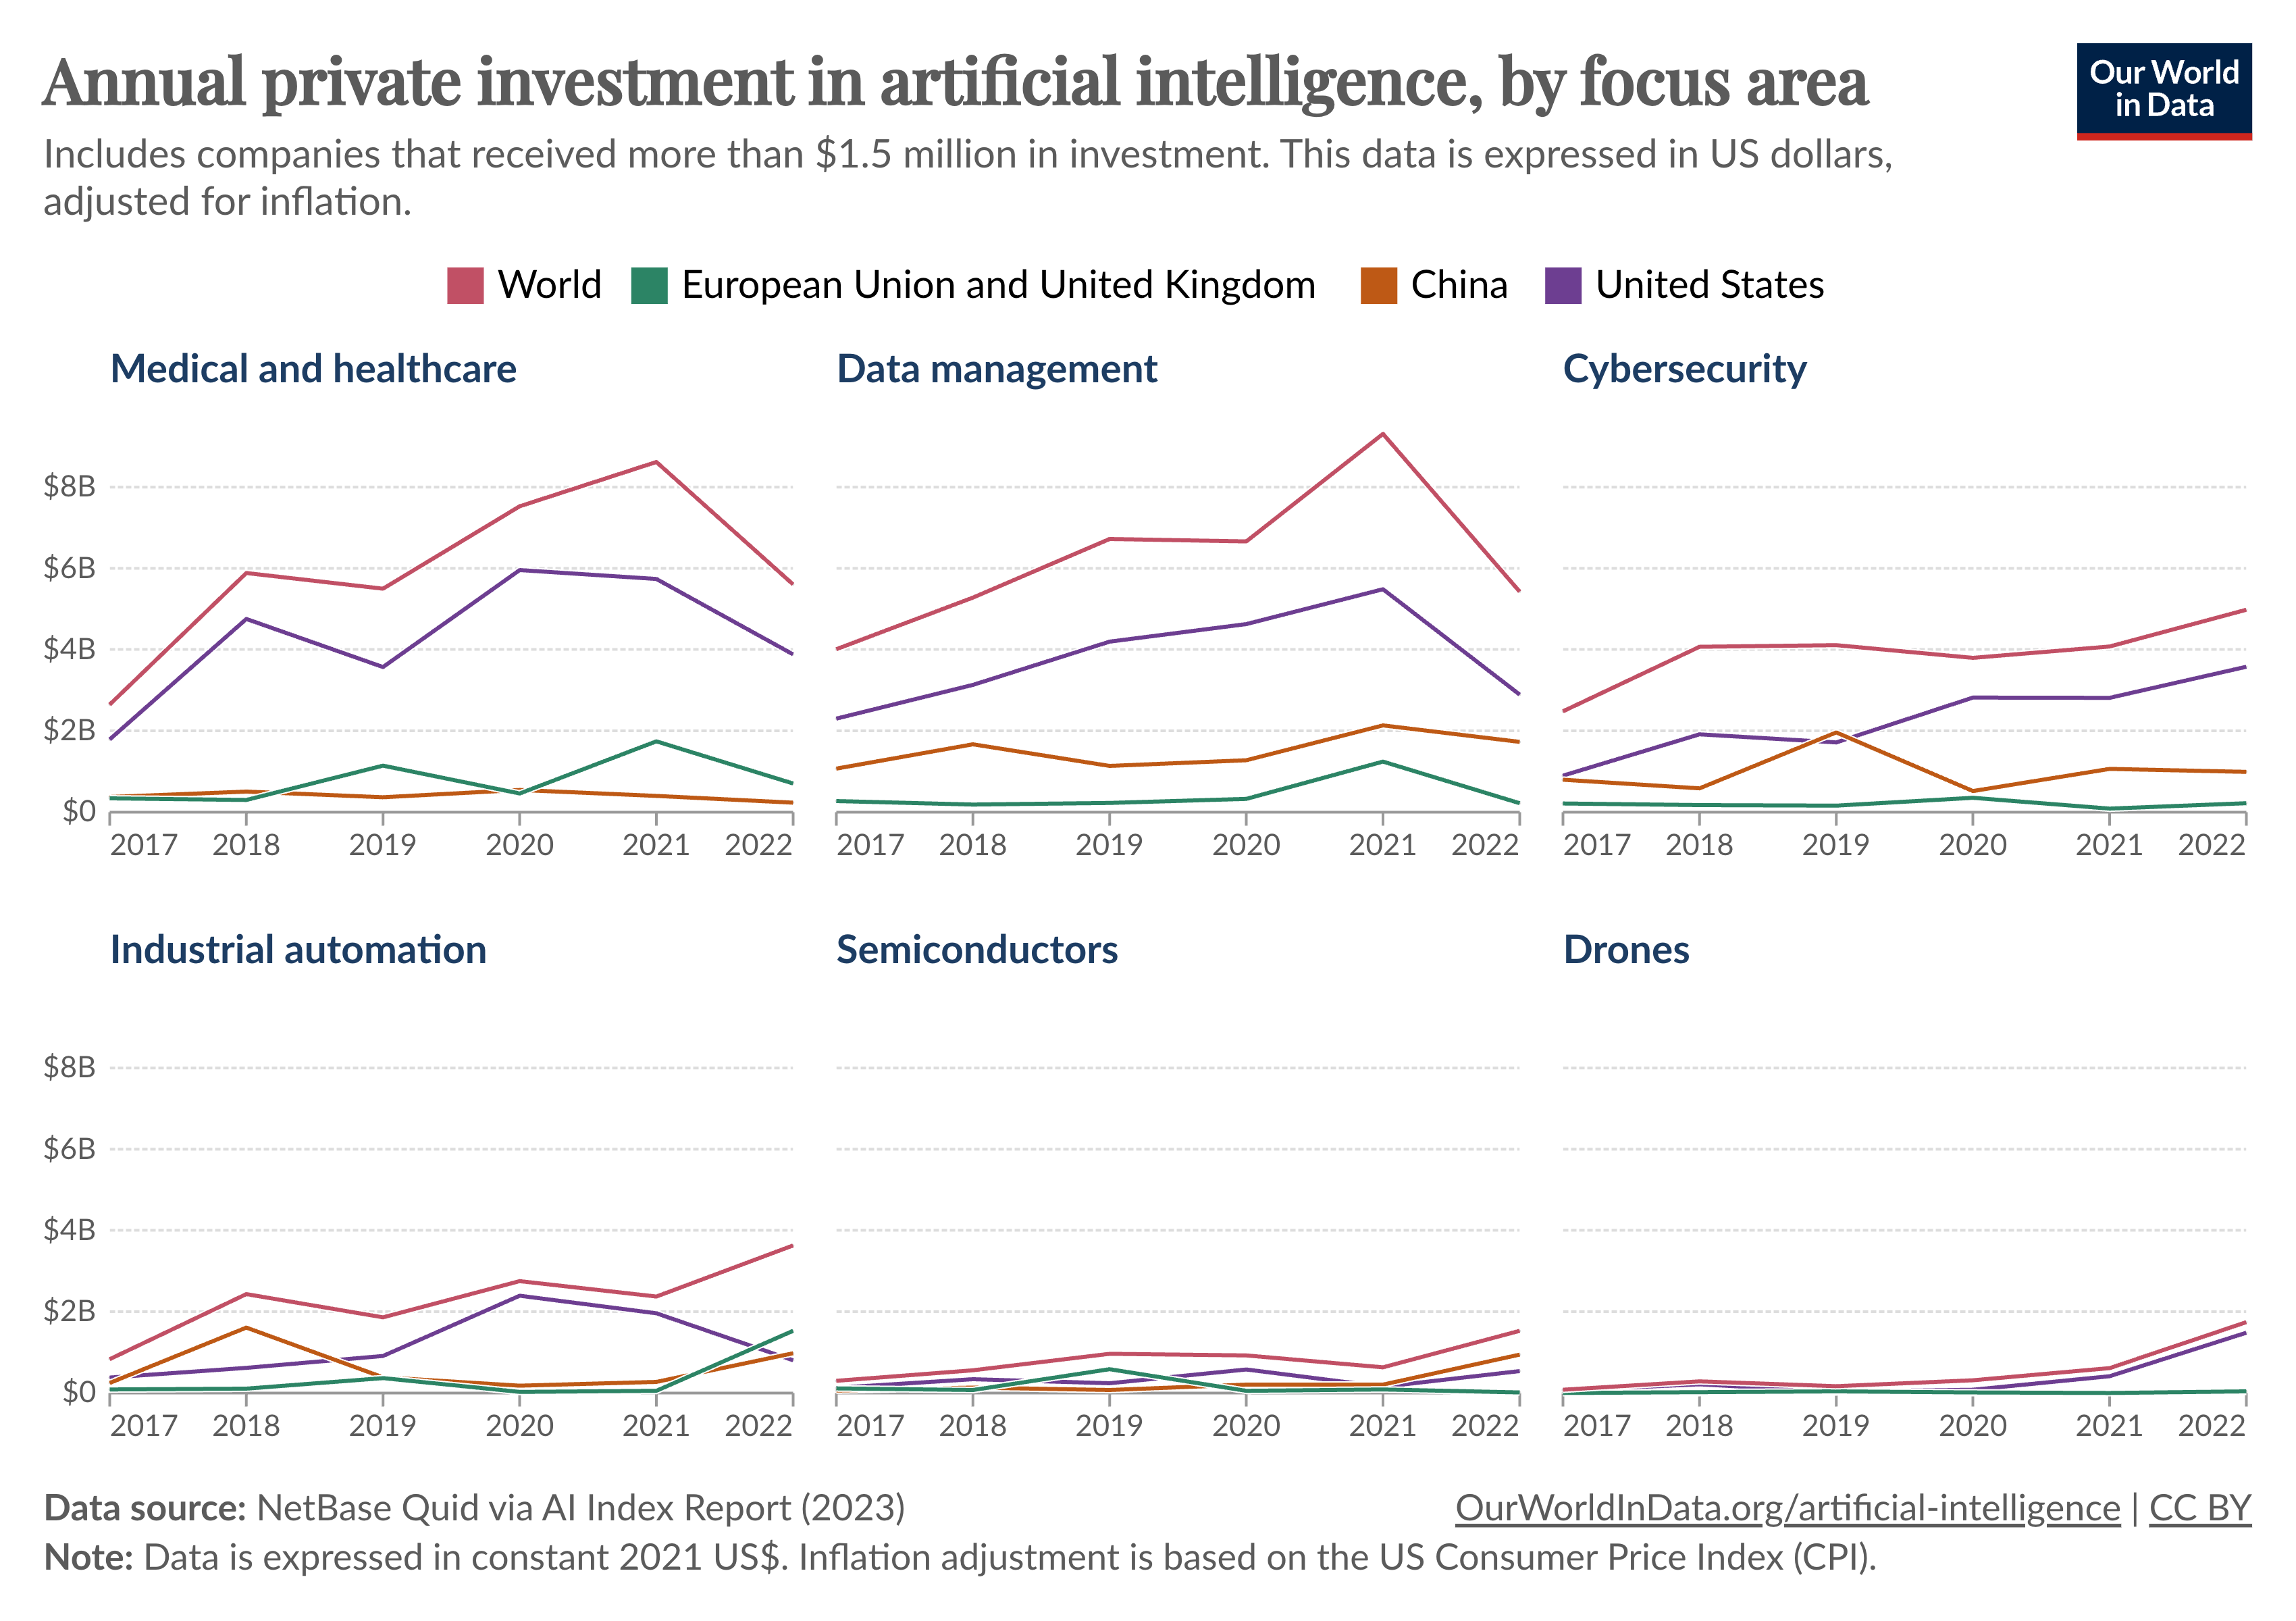
\includegraphics[width=\linewidth]{./data/investment_by_area.png}
        \caption{Annual investment in AI by area}
        \label{fig:views_ai_impact}
    \end{minipage}
\end{figure}


% 隐私和数据保护
\section{Privacy and data protection}
In the realm of Healthcare AI, the protection of patient privacy and data is paramount. 
Patients express concerns about the use of their sensitive information, such as medical 
records and test results, which are stored in hospital databases. They question the duration 
of data storage, access by staff, purposes of data use, and potential for unauthorized sharing \cite{JayasundaraETHICALISSUESSURROUNDING}. 
Although electronic records offer increased security compared to paper files, there remains a 
risk of cyberattacks and internal visibility. The implications of data breaches are profound, 
affecting personal life through potential bullying, increased insurance costs, and job loss 
due to disclosed medical history \cite{Thapa2021PrecisionHealthData}. Therefore, ensuring robust data protection measures and 
transparency in data handling is essential for maintaining trust in healthcare services.


% 信任
\section{Transparency and Trust}
The pervasive "black box" nature of AI algorithms fuels transparency and trust issues 
in Healthcare AI (HCAI). The public's apprehension is amplified by concerns over HCAI's 
recommendations for diagnosing and treating medical conditions, despite physician oversight \cite{esmaeilzadehPatientsPerceptionsHuman2021}. 
This skepticism is particularly strong among older individuals and those with lower economic 
status, who fear AI may bring more harm than good. The lack of direct experience with HCAI 
and a basic understanding of AI contribute to a global sentiment of unease about AI's societal 
impact in the coming decades.

\begin{figure}[H]
    \centering
    \begin{minipage}[t]{0.48\linewidth}
        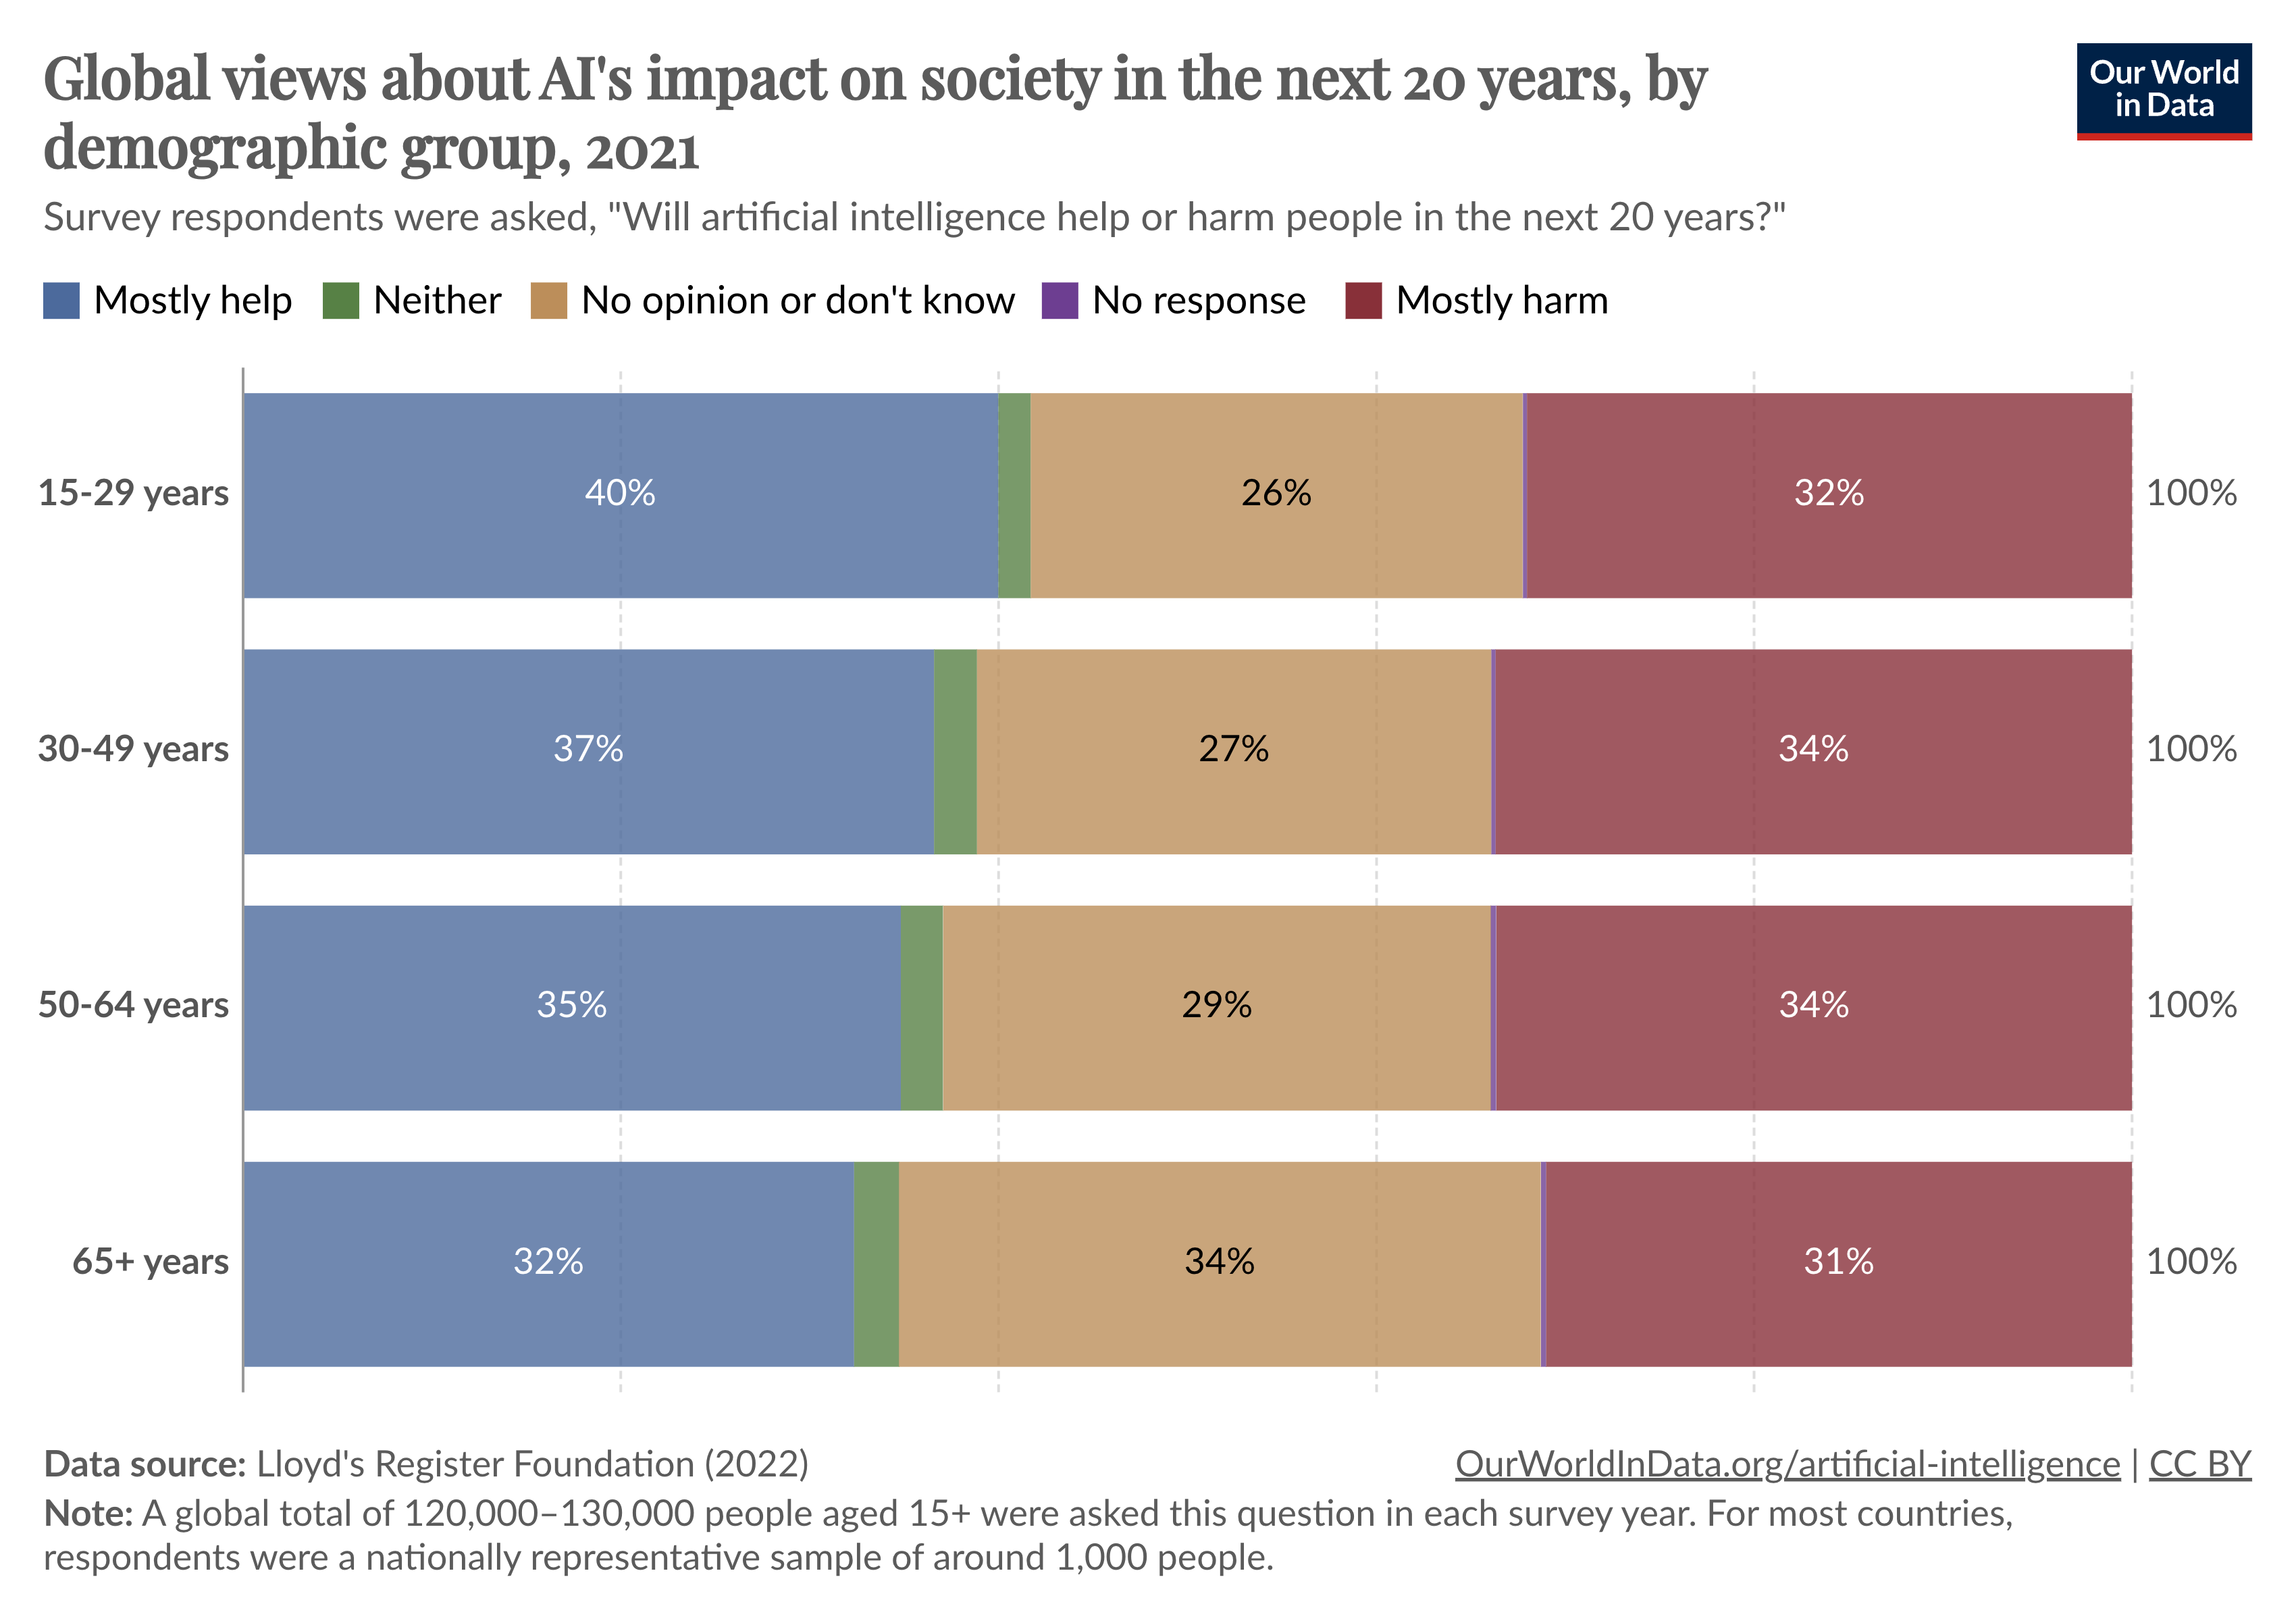
\includegraphics[width=\linewidth]{./data/influence_by_ages.png}
        \caption{Views on AI's impact on society by ages}
        \label{fig:investment}
    \end{minipage}\hfill
    \begin{minipage}[t]{0.48\linewidth}
        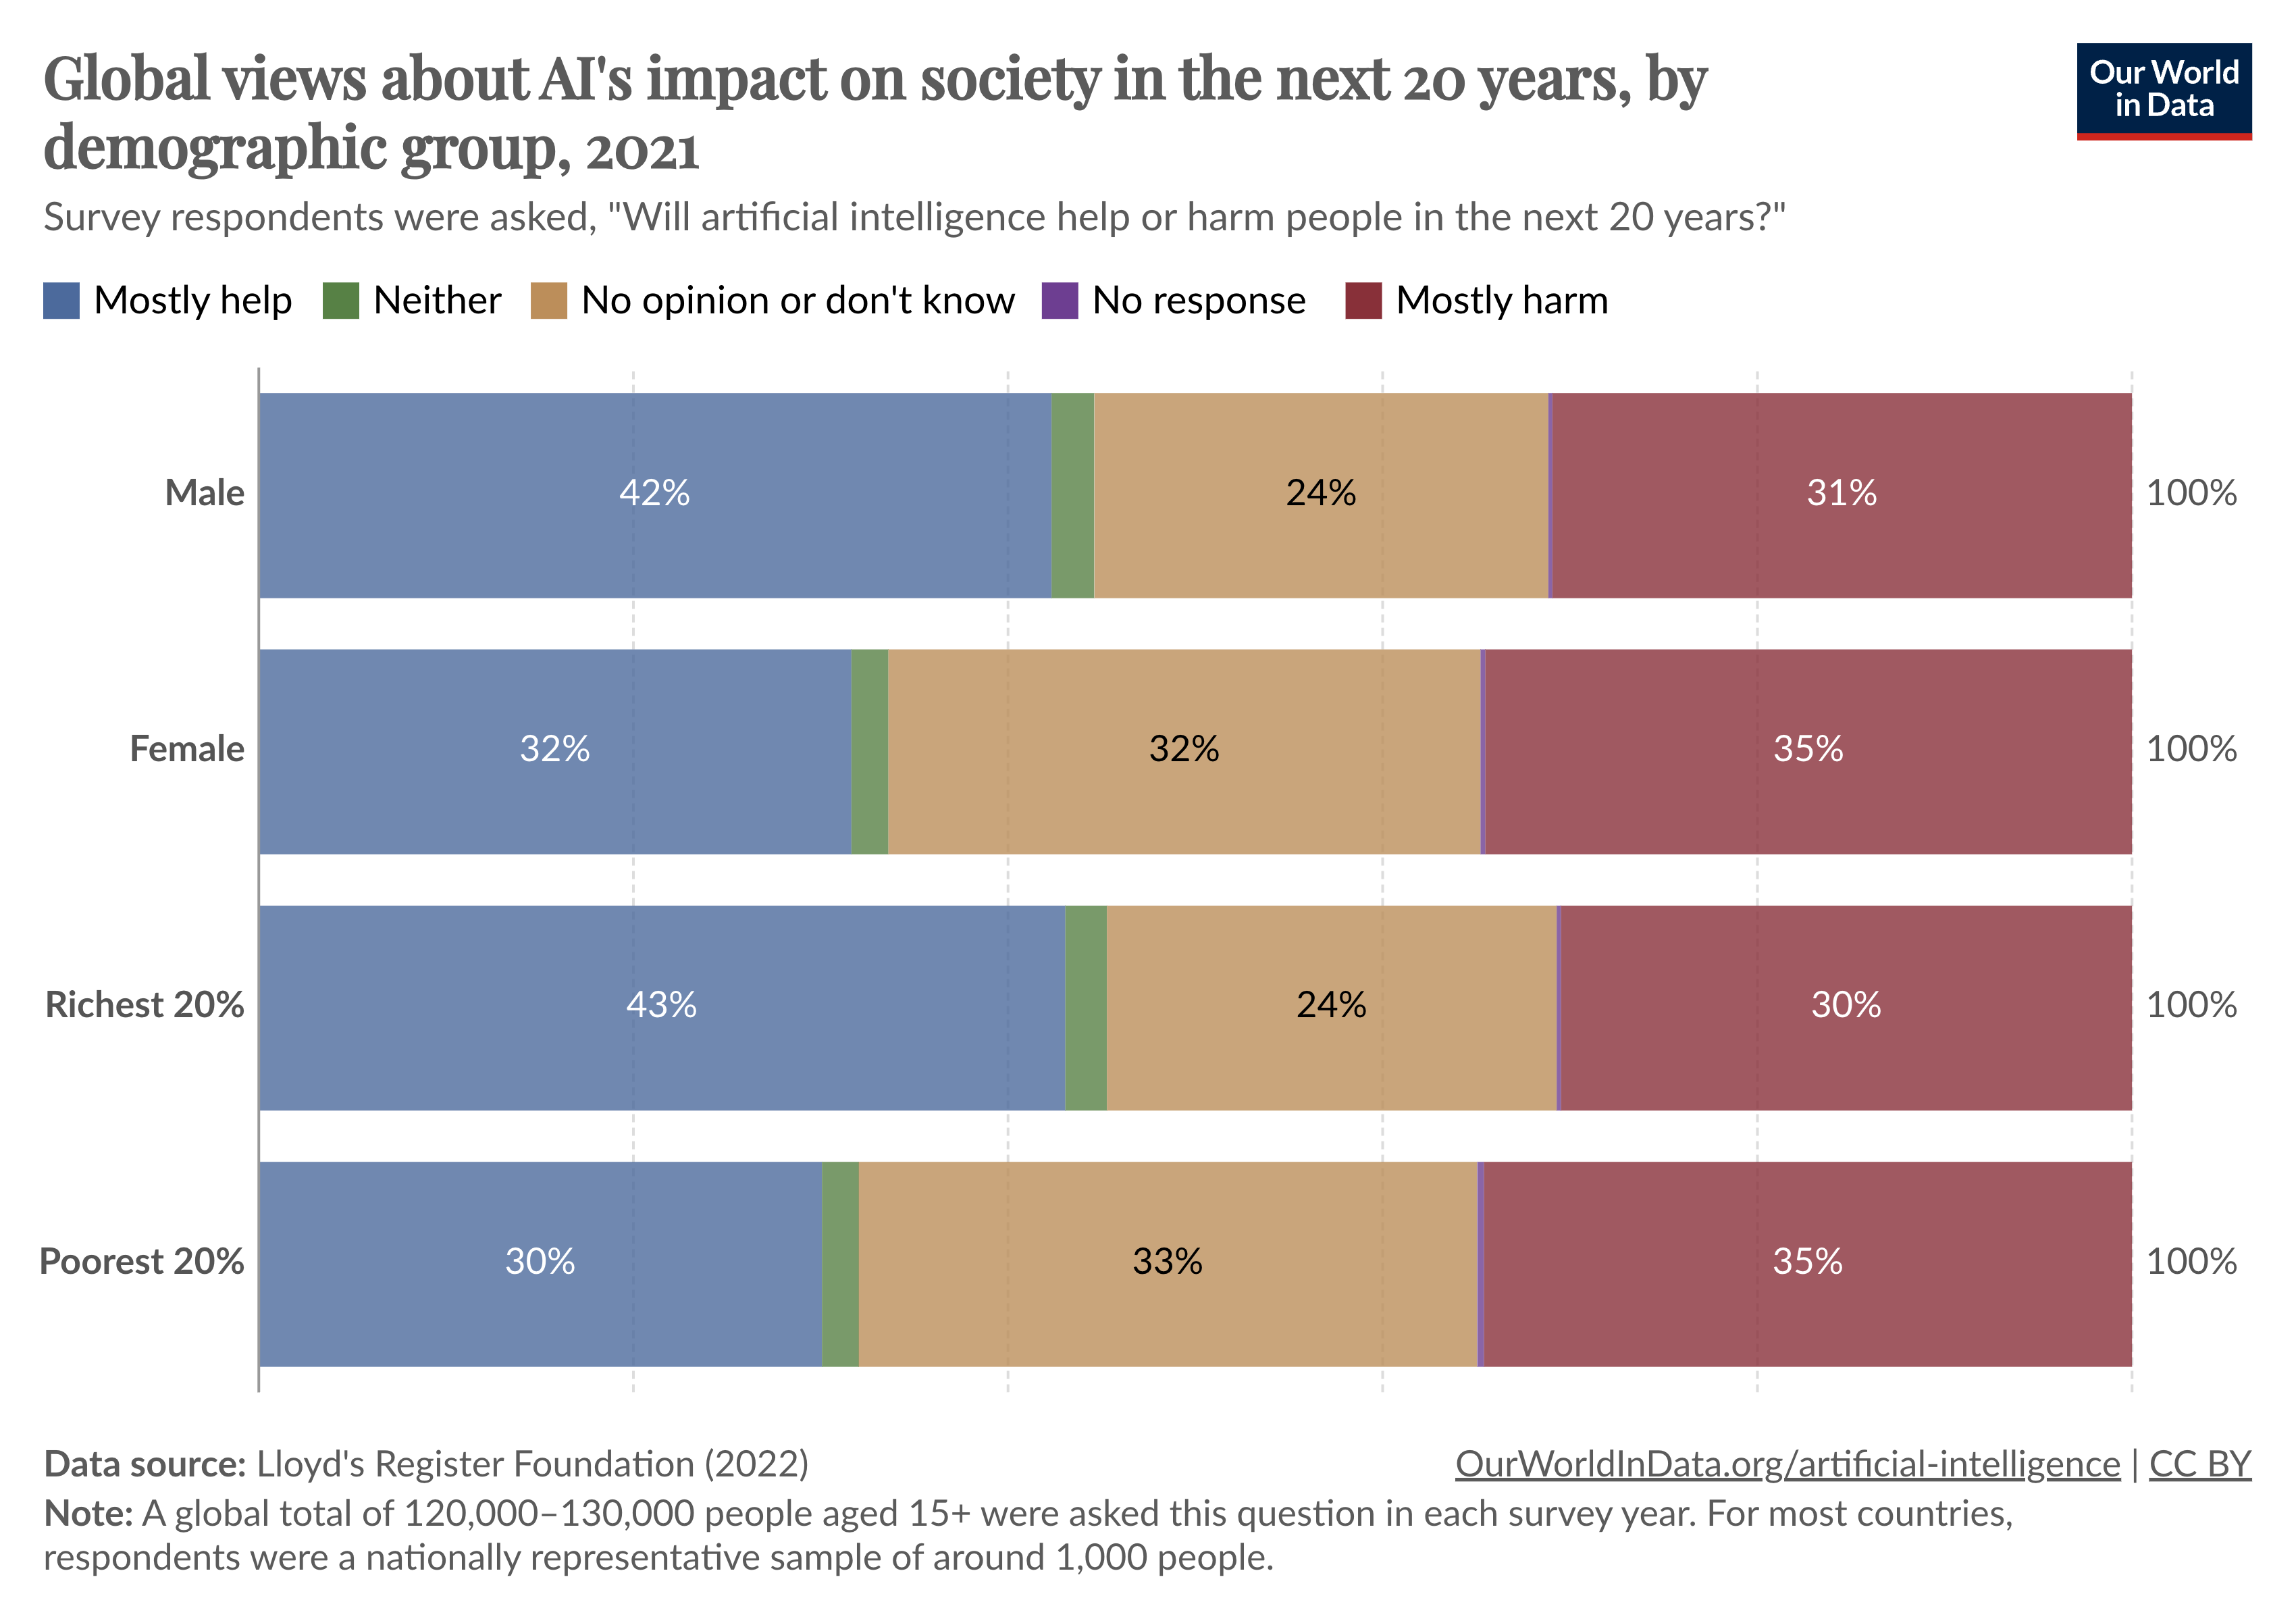
\includegraphics[width=\linewidth]{./data/influence_by_demographic_group.png}
        \caption{Views on AI's impact on society by gender and wealth}
        \label{fig:views_ai_impact}
    \end{minipage}
\end{figure}


% 责任和问责
\section{Responsibility and Accountability}
Historically, healthcare prioritized the doctor-patient relationship, focusing on shared decision-making 
to tailor care plans to patient needs. Clinical decisions, grounded in patient information, were the sole 
responsibility of doctors \cite{Smith2021ClinicalAIOpacity}. The emergence of "black box" AI tools, with their opaque algorithms, now poses 
a challenge to this collaborative process by limiting patient autonomy due to a lack of explainability. 
Although AI could allow doctors more time for patient interaction, its benefits are constrained if AI's 
recommendations cannot be fully explained. The integration of such technologies raises concerns about 
new sources of medical errors in a field where mistakes have grave consequences.


\section{suggestings}
(1) Implement encryption, restrict access, enhance transparency, and educate on policies to boost patient trust and safeguard privacy in healthcare AI.
\\(2) To address transparency and trust in HCAI, it's vital to enhance AI explainability, involve diverse patient groups in AI development, and provide AI literacy education.
\\(3) Establishing robust AI-assisted decision-making protocols, supported by rigorous oversight, is critical to minimizing medical errors

 



\section{Conclusion}
This article analyzes the ethical issues of artificial intelligence in healthcare from three 
perspectives: patient privacy and data protection, public trust in AI, and physician responsibility 
and accountability, offering corresponding recommendations. The ethical dilemmas in healthcare AI 
largely stem from a lack of understanding of new technologies and unclear regulatory guidelines. 
The emergence of new technologies often disrupts existing systems, and the inevitable disruption 
caused by AI in traditional healthcare necessitates regulatory guidance to ensure a smooth transition to new systems.




% \begin{figure}[h]
%     \centering
%     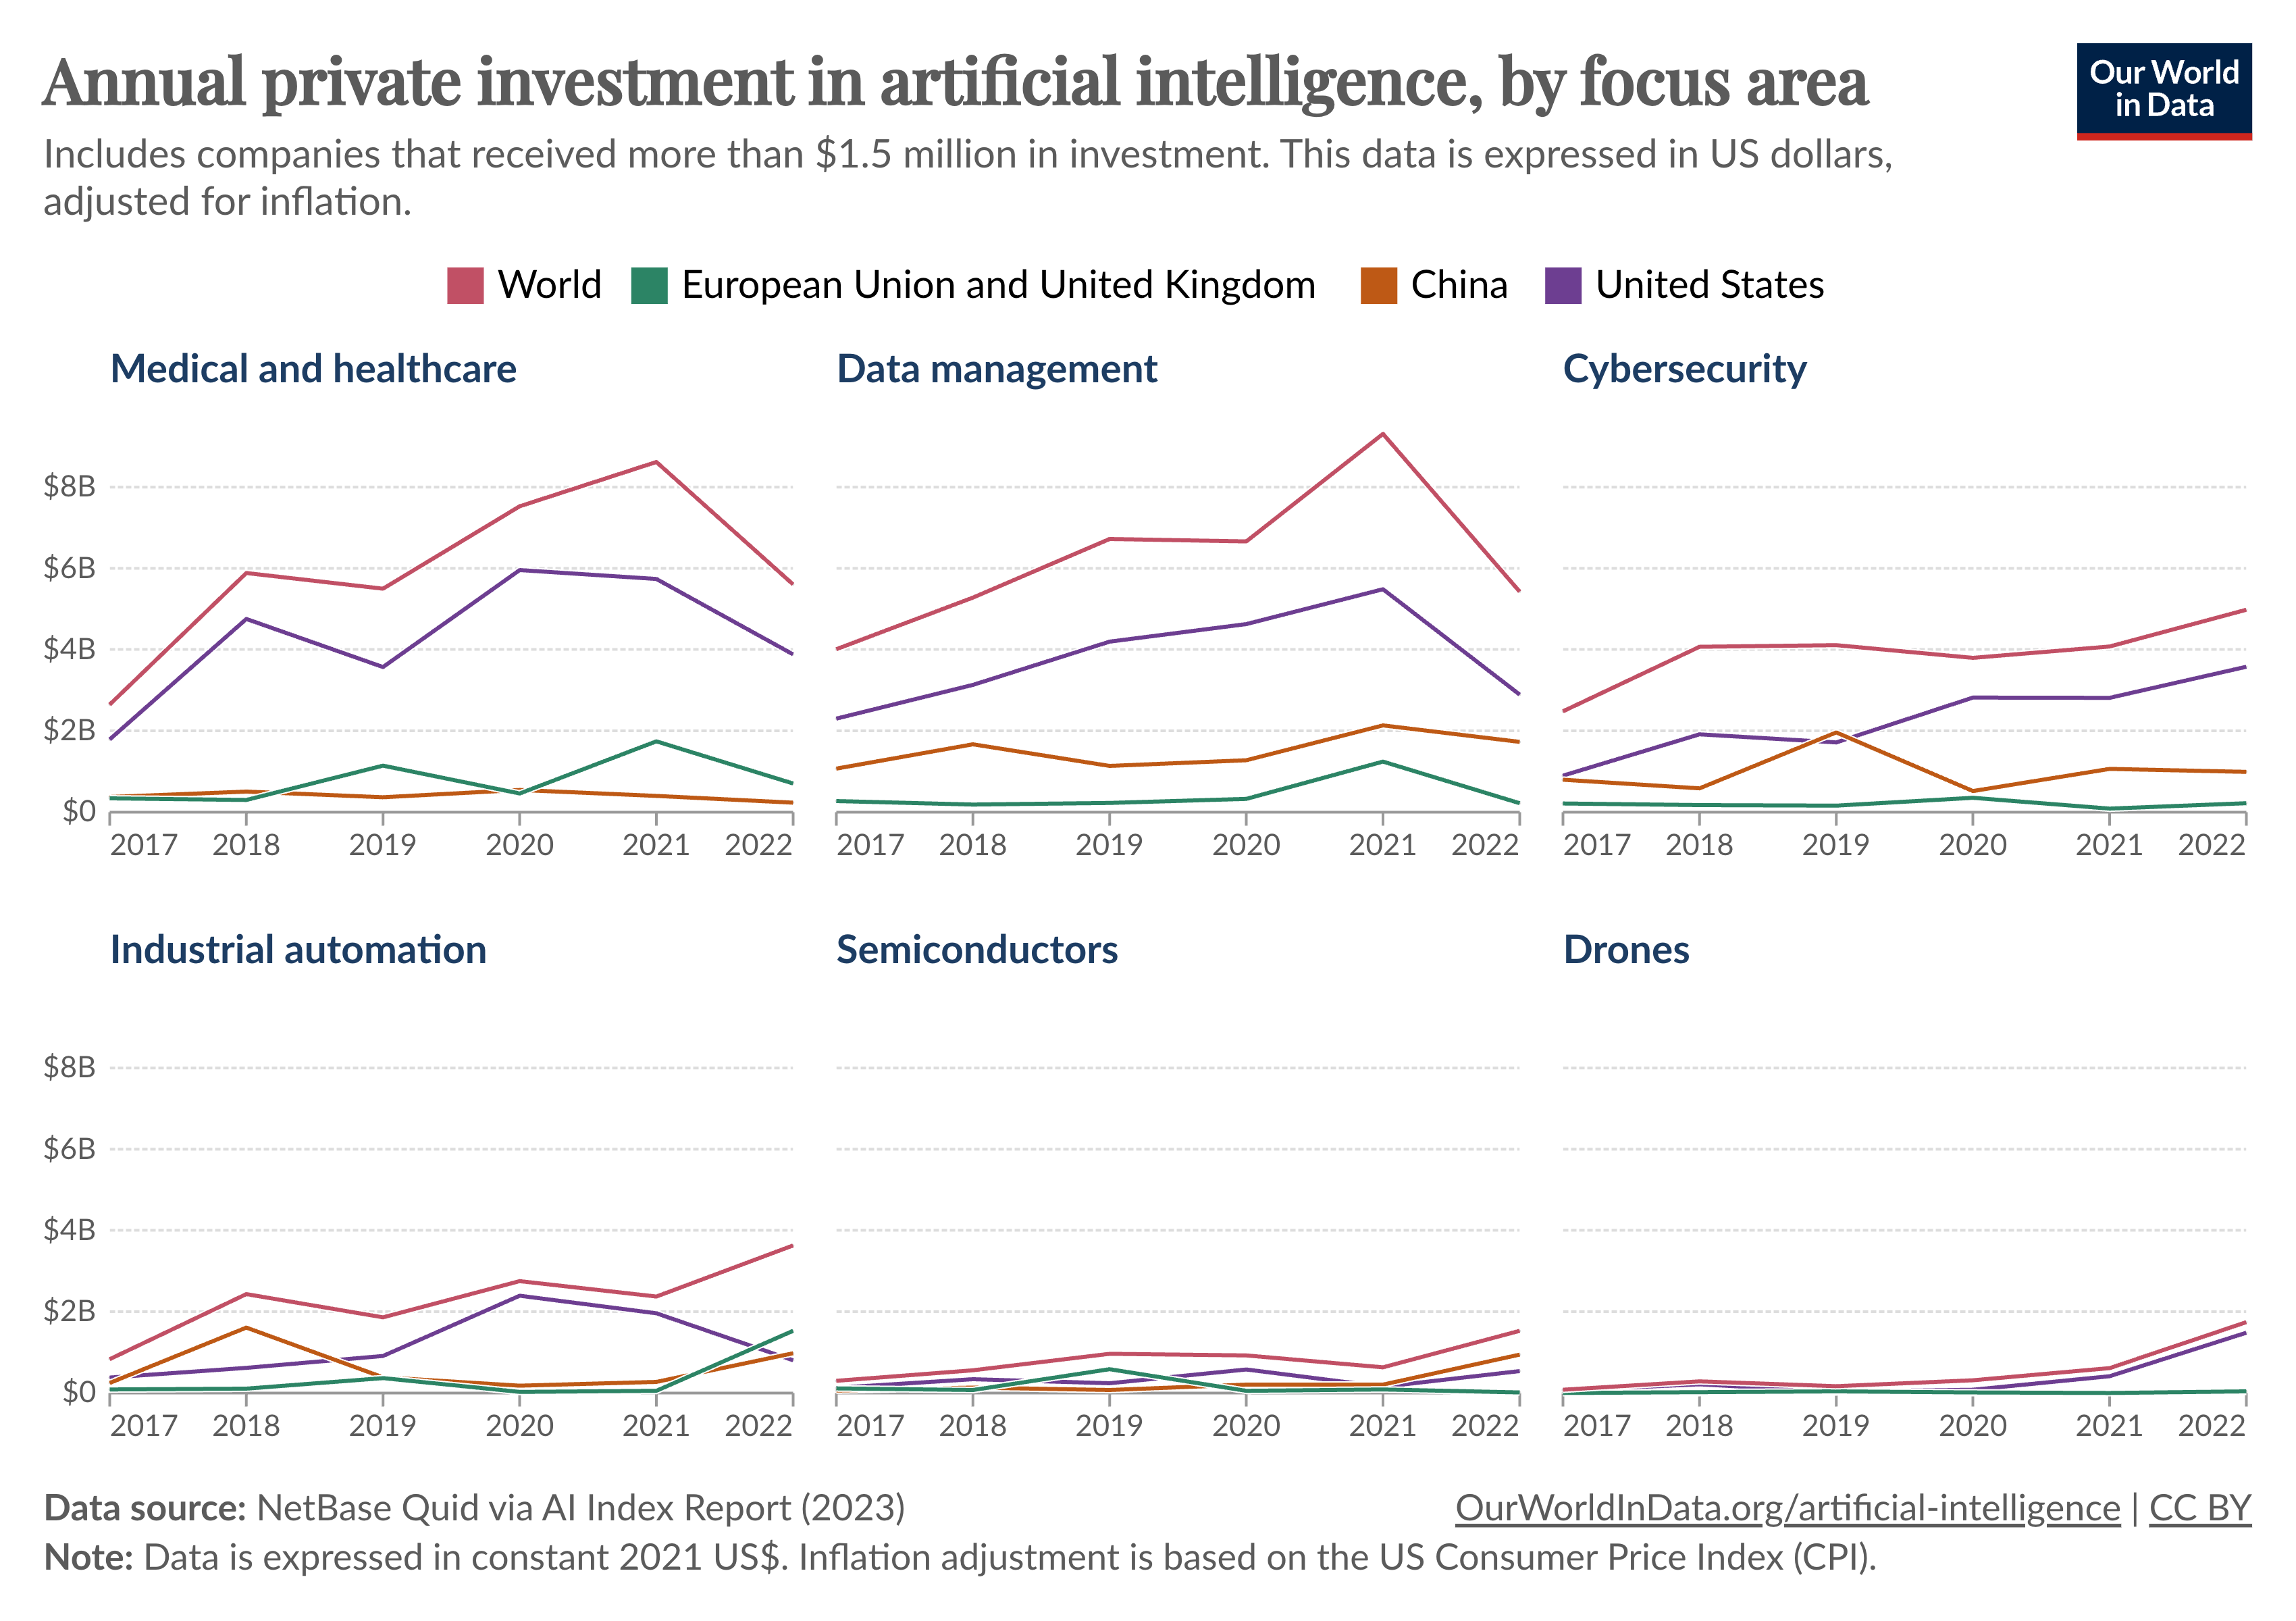
\includegraphics[width=0.9\textwidth]{./data/investegatement.png}
%     \caption{This is the title}
%     \label{fig:my_picture}
% \end{figure}



% \begin{figure}[h]
%     \centering
%     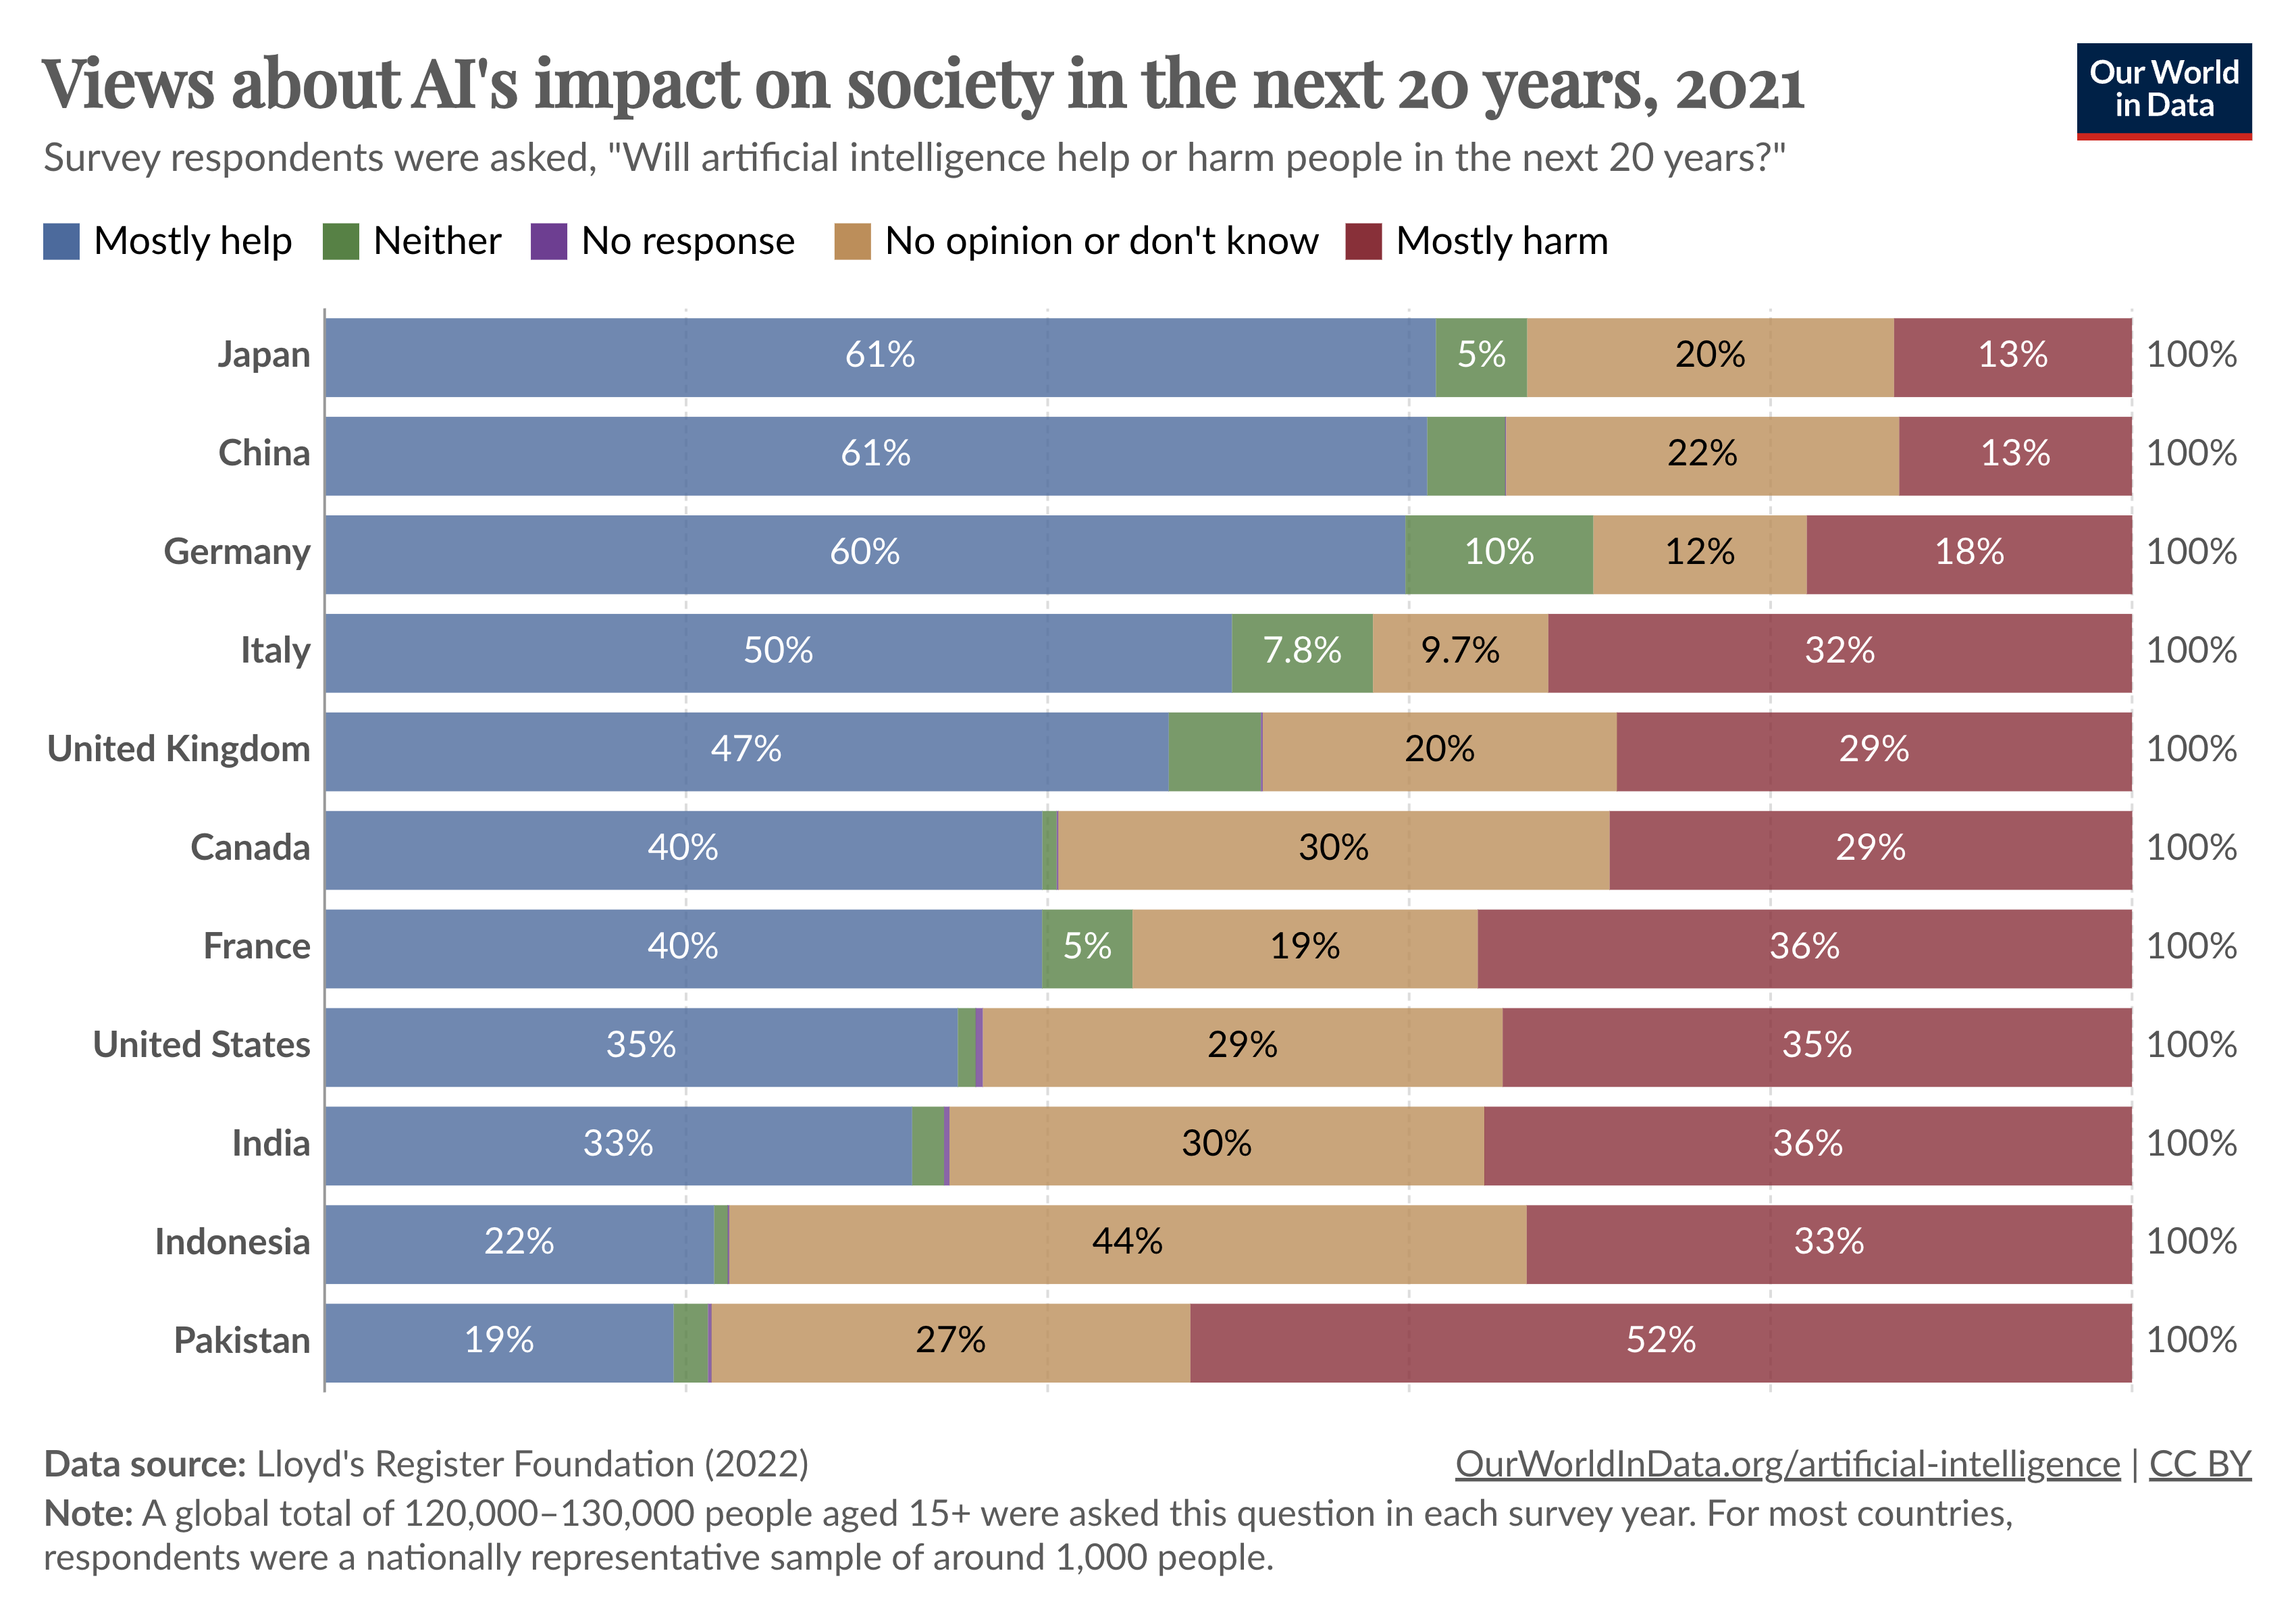
\includegraphics[width=0.9\textwidth]{./data/influence.png}
%     \caption{This is the title}
%     \label{fig:my_picture}
% \end{figure}
















%----------------------------------------------------------------------------------------

\bibliographystyle{unsrt} % This specifies the style of the bibliography
\bibliography{/Users/dengkai/workspace/papers/latex/config/ref} % This should match the name of your .bib file without the extension
\end{document}

